\chapter{Experimenty}

V této kapitole prezentujeme přehled výsledků různých architektur pro \uloha{extrakci melodie}, trénované nad datasetem \dataset{MedleyDB}. Data byla rozdělena na trénovací, validační a testovací množinu tak, aby skladby od jednoho interpreta náležely právě do jedné z množin. Využili jsme existujícího rozdělení používaného v článcích \cite{Bittner2017} a \cite{DBasaranSEssid2018}, validační i testovací výsledky jsou tedy díky tomu porovnatelné s výsledky uvedenými v článcích.

Pro odhad \uloha{výšky tónů} porovnáváme architektury inspirované pracemi \cite{Kim2018}, \cite{Oord2016} a \cite{Bittner2017}. V prvním případě jde o architekturu CREPE původně navrženou pro sledování výšky tónů v jednohlasých nahrávkách. \cite{Oord2016} používají WaveNet složený z dilatovaných konvolucí pro generování lidské řeči. \cite{Bittner2017} používá hlubokou konvoluční síť pro kompletní přepis nahrávek i pro přepis melodie. 

Pro \uloha{detekci melodie} pak srovnáváme jednoduchou metodu práhování a složitější samostatný modul, založený na hlubokých neuronových sítích.

\section{Architektura CREPE}

První sada experimentů se zakládá na architektuře popsané v článku od \cite{Kim2018} použité pro \uloha{sledování jednohlasu}. Jak blíže popisujeme v kapitole \nameref{cha:souvisejici}, cílem monopitch trackingu je určit konturu základní frekvence melodického nástroje v jednohlasé nahrávce. Tato nahrávka se zpravidla skládá ze směsi čistého signálu hlasu a šumu v pozadí. Pokud však rozšíříme pojem šumu v pozadí tak, aby zahrnoval i melodický doprovod, pak dostáváme polyfonní signál, tedy vstupní signál pro metody \uloha{extrakce melodie}.

Jinými slovy je \uloha{sledování jednohlasu} speciálním případem \uloha{extrakce melodie} a tudíž přinejmenším stojí za zkoušku pokusit se tuto architekturu pro extrakci využít. Mimo to jednohlasé stopy často obsahují přeslech ostatních nástrojů, pokud nahrávka vznikala při společném hraní ve studiu, tudíž by model trénovaný na vícehlasé mixech mohl být robustní vůči tomuto druhu rušení. 

\begin{figure}[h]\centering
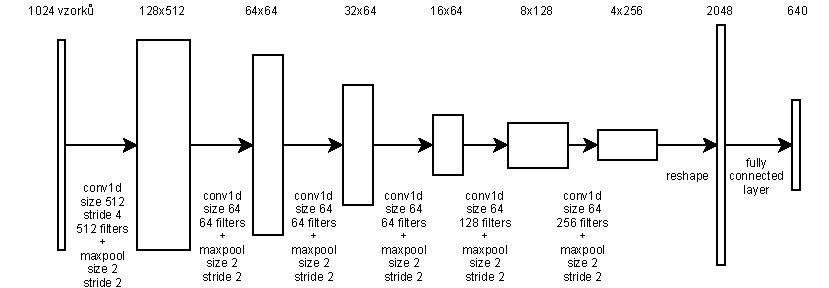
\includegraphics{../img/crepe_arch}
\caption{Diagram architektury CREPE, multiplikační koeficient 16x.}
\label{obr:wavenet_dilated}
\end{figure}

Architektura CREPE se skládá ze šesti konvolučních a pooling vrstev, pro regularizaci používá batch normalization a dropout po každé konvoluční vrstvě, jako nelineární aktivace je použita funkce ReLU. Po konvolucích následuje výstupní plně propojená vrstva, jako finální aktivační funkce je použita sigmoida. Vstupem modelu je okno o velikosti 1024 vzorků jednokanálového audio signálu, převzorkovaného na 16 kHz. Před první konvolucí je signál normalizován tak, aby každé jednotlivé vstupní okno mělo střední hodnotu 0 a směrodatnou odchylku 1. Podrobnější popis modelu je naznačen na obrázku.

Výsledný vektor o 640 složkách aproximuje pravděpodobnostní rozdělení výšky základní frekvence uprostřed vstupního okna, přičemž tento vektor pokrývá rozsah od noty $C_{-1}$ po $G_{9}$, mezi dvěma sousedními predikovanými tóny je vzdálenost 20 centů. Výšky tónů v centech označíme $\cent_1, \cent_2, \dots, \cent_{640}$. Rozsah tedy bezpečně pokrývá obvyklé hudební nástroje a na jednu notu připadá 5 složek (tónů) výsledného vektoru.

    $$\cent(f) = 1200 \log_2{\frac{f}{f_{\mathrm{ref}}}}$$

Pro trénování modelu potřebujeme také cílové diskrétní pravděpodobnostní rozdělení základní frekvence tónu. Jako cílovou pravděpodobnostní funkci použijeme normální rozdělení se střední hodnotou v bodě cílové základní frekvence $\cent(f_{\mathrm{ref}})$ a se směrodatnou odchylkou 25 centů. Toto rozdělení diskretizujeme tak, aby měl cílový vektor stejné dimenze jako odhadovaný.

    $$y_i = \frac{1}{\sqrt{2 \pi \sigma^2}}\exp{(-\frac{(\cent_i - \cent_{\mathrm{ref}})^2}{2 \sigma^2})}$$

Převod z pravděpodobnostní reprezentace výstupního vektoru na konkrétní hodnotu výšky noty provedeme pomocí výpočtu střední hodnoty výstupní distribuce. Jelikož by při výpočtu střední hodnoty ale hodnotu výsledné výšky tónu ovlivňoval i doprovod, který se na výstupním vektoru objevuje, počítáme střední hodnotu pouze z okolí maxima výstupu. Tím zajistíme, že získáme střední hodnotu gaussiánu náležícímu pouze jednomu tónu.

    $$ \left. \hat{\cent} = \sum_{\scaleto{i, \lvert \cent_i - \cent_m \rvert < 50}{8pt}} {\hat{y}_i \cent_i} \middle/ \sum_{\scaleto{i, \lvert \cent_i - \cent_m \rvert < 50}{8pt}} \hat{y}_i \right., m = \mathrm{argmax}_i(\hat{y}_i)$$

Optimalizovaná loss funkce modelu $\mathcal{L}(\mathbf{y}, \mathbf{\hat{y}})$ se počítá jako vzájemná korelace mezi vektorem cílových pravděpodobností $y$ a výstupním vektorem $\hat{y}$.

    $$\mathcal{L}(\mathbf{y}, \mathbf{\hat{y}}) = \sum_{i = 1}^{640}{(-y_i\log\hat{y}_i - (1-y_i)\log(1-\hat{y_i}))}$$

Optimalizace probíhá pomocí algoritmu Adam \citep{Kingma2014} s parametrem learning rate $0.0002$.

\begin{table}[h!]

\centering
%%% Tabulka používá následující balíčky:
%%%   - booktabs (\toprule, \midrule, \bottomrule)
%%%   - dcolumn (typ sloupce D: vycentrovaná čísla zarovnaná na
%%%     desetinnou čárku
%%%     Všimněte si, že ve zdrojovém kódu jsou desetinné tečky, ale
%%%     tisknou se čárky.
%%% Dále používáme příkazy \pulrad a \mc definované v makra.tex
    \begin{tabular}{l@{\hspace{1.5cm}}rrrrrrr}
    \toprule
    {}         &  \textbf{1.}   &  \textbf{2.}  &  \textbf{3.}  &  \textbf{4.}  &  \textbf{5.}   &  \textbf{6.}  &  \textbf{Celk. parametrů} \\
    \midrule
    CREPE 4x   &  128  &  16  &  16  &  16  &  32   &  64  &  $558\,240$ \\
    CREPE 8x   &  256  &  32  &  32  &  32  &  64   &  128 &  $177\,1200$ \\
    CREPE 16x  &  512  &  64  &  64  &  64  &  128  &  256 &  $6\,163\,200$ \\
    \bottomrule
    \end{tabular}

\caption{Počty filtrů v konvolučních vrstvách v architektuře CREPE v závislosti na multiplikačním koeficientu.}\label{tab:crepe_dimensions}

\end{table}

% rozepsat:
% - obhajoba raw signálu

% diskuze:
% - převzorkování na 16kHz
% - normalizace vstupu
% - formulace jako klasifikační úloha, nikoli regresní
% - je lepší odhadovat opravdové pravděpodobnostní rozdělení a nebo jejich škálované? (přijde mi, že kvůli sigmoid aktivaci bude jednodušší 1.0 = Truth, protože ty vstupní logity do sigmoid aktivace můžou být crazyshit velký)
% - crepe model - např. nedává vůbec smysl velikost kernelu 64 v posledních vrstvách, zbytečně se tam přidávají nuly jako padding


\subsection{Replikace výsledků CREPE}

Abychom ověřili správnost implementace architektury CREPE pro sledování jednohlasu, spustíme model na syntetických, jednohlasých datech \emph{MDB-stem-synth}, která byla zvěřejněná spolu s článkem od \cite{Salamon2017}.

Na rozdíl od článku \cite{Kim2018}, ve kterém autoři používají pro celkové vyhodnocení architektury pětinásobnou křížovou validaci, jsme použili pouze jednu trénovací a testovací množinu. Zásadní rozdíly mezi implementacemi modelu jsme na základě článku a veřejně dostupného kódu neobjevili.

Po jedné epoše trénování model dosáhl na testovací množině $98.6\%$ přesnosti odhadu výšky. \cite{Kim2018} uvádí přesnost modelu $97\%$. V jejich případě jde o průměrný výsledek pěti nezávislých běhů trénování a testování na různě rozdělených datových množinách. Rozdíl v dosažených přesnostech přičítáme odlišné evaluační strategii.

\begin{table}[h!]

\centering
    \begin{tabular}{llrr}
    \toprule
    Metrika & Práh & Průměrná hodnota & Hodnota \cite{Kim2018} \\
    \midrule
    RCA & 50 centů & 0.988 & 0.970 \\
    RPA  & 50 centů & 0.986 & 0.967 \\
    RPA  & 25 centů & 0.975 & 0.953 \\
    RPA  & 10 centů & 0.937 & 0.909 \\
    \bottomrule
    \end{tabular}
\caption{Výsledky pokusu o replikaci. Přesnosti nejsou přímo srovnatelné kvůli různým evaluačním strategiím.}\label{tab:crepe_dimensions}

\end{table}


Při replikaci experimentu jsme narazil na důležitost správného promíchání dat. Framework Tensorflow použitý pro trénování promíchává data vždy pomocí bufferu pevné velikosti pro dvojice vstupů a cílových výstupů. V praxi je však potřeba buď nastavit buffer na velikost větší než je celková velikost datasetu, a nebo implementovat vlastní míchání přes všechna dostupná data. Při nedostatečně promíchaných datech totiž trénovací dávka (batch) není reprezentativní pro celý dataset, ale pouze pro jeho podmnožinu, což se negativně projevuje kolísající validační přesností modelu.

\subsection{CREPE pro extrakci melodie}

Jako první experiment \uloha{extrakce melodie} z polyfonních dat spustíme nezměněnou architekturu CREPE, v následujících experimentech se tuto baseline pokusíme překonat. Abychom urychlili trénování následujících experimentů, přesnost určíme pro sítě s různou kapacitou. Pokud se výsledky při různých kapacitách nebudou příliš lišit, můžeme experimenty provádět s architekturou s nižší kapacitou a tím snížit trénovací čas. Kapacity upravíme pomocí multiplikačního koeficientu počtu filtrů u všech konvolučních vrstev, počty filtrů jsou uvedeny v tabulce \ref{tab:crepe_dimensions}.

% TODO: diskuse o under a overfittingu

\begin{table}[h!]

\centering
    \begin{tabular}{l@{\hspace{1.5cm}}rr}
    \toprule
    \textbf{Model}      &  \textbf{RPA}    &  \textbf{RCA} \\
    \midrule
    CREPE 4x   &  0.634  &  0.753 \\
    CREPE 8x   &  0.661  &  0.766 \\
    CREPE 16x  &  0.666  &  0.771 \\
    \bottomrule
    \end{tabular}
\caption{Výsledky experimentu s různými kapacitami modelu.}\label{tab:crepe_dimensions}

\end{table}

Z validačních výsledků po $200\,000$ iteracích (přibližně 6 epoch) vidíme, že se výsledek modelů CREPE 8x a CREPE 16x liší řádově o desetiny procentních bodů. Přitom model s větší kapacitou se trénuje o 35\% delší dobu. Proto pro další srovnávání zvolíme architektury s multiplikačním koeficientem 8, modely s dobrými výsledky případně přetrénujeme s vyšší kapacitou.

\subsection{Vliv rozlišení diskretizace výšky noty}

Otestujeme nastavení granularity výstupního vektoru. V článku \cite{Kim2018} se totiž důvod volby pěti frekvencí na notu nediskutuje. Intuitivně by však mělo vyšší rozlišení spíše pomáhat, důvodem je, že nástroje a zejména lidský hlas se často při hraní odchylují od přesných frekvencí hraných not a vyšší rozlišení tyto odchylky může lépe zachytit. Ve výsledku by pak síť s jemnějším výstupem měla dělat méně chyb, kde se skutečná a výstupní hodnota liší o jeden půltón.

    \begin{tabular}{llrr}
    \toprule
    Kapacita & Diskretizace &  RPA &  RCA \\
    \midrule
     4x &        hrubá      & 0.606 & 0.708 \\
     4x &        jemná      & 0.634 & 0.753 \\
     8x &        hrubá      & 0.614 & 0.724 \\
     8x &        jemná      & 0.661 & 0.766 \\
    16x &        hrubá      & 0.612 & 0.711 \\
    16x &        jemná      & 0.666 & 0.771 \\
    \bottomrule
    \end{tabular}

% TODO: Přidat graf

Jak můžeme pozorovat na výsledných hodnotách, jemná granularita výstupu jednoznačně zlepšuje přesnost sítě. Abychom ověřili domněnku, že vyšší rozlišení pomáhá zmenšit počet chyb o půltón, vytvoříme histogram vzdáleností cílového a odhadovaného tónu. V tomto histogramu by pak měl být zřetelný pokles v příslušných třídách. Podle histogramu se počet chyb o půltón mezi zkoumanými modely liší téměř o polovinu, zlepšení tohoto druhu chyb je tedy podstatné.

\subsection{Vliv rozptylu cílové pravděpodobnostní distribuce výšky noty}

Podle \cite{Bittner2017} pomáhá cílová distribuce s vyšším rozptylem snížit penalizaci sítě za téměř korektní odhady výšek tónů. Mimo to u dostupných dat často nejsou anotace naprosto perfektní, jisté rozostření hranice anotace tudíž pomáhá i v případě nepřesné cílové anotace, síť pak není tolik penalizována za svou případnou správnou odpověď. 

V článku se však nediskutuje nastavení směrodatné odchylky na 20 centů, \cite{Kim2018} používá odchylku 25 centů a není na první pohled zřejmé, jaká je optimální hodnota. Příliš vysoký rozptyl způsobí, že síť bude tolerovat více chyb o půltón, příliš nízký rozptyl naopak penalizuje i téměř správné odhady. Intuitivně se nejlepší nastavení pravděpodobně bude pohybovat kolem používaných 25 centů, jelikož to je hranice chybné klasifikace, na druhou stranu optimální hodnota jistě bude závislá na nastavení rozlišení výstupního vektoru, jelikož nižší rozlišení bude jistě vyžadovat vyšší hodnotu rozptylu (v extrémním případě rozptylu blížícího se k nule a cílové frekvence mimo kvantizační hladiny by vzniklý cílový vektor nemusel obsahovat žádné ostré maximum).

Poznamenám také technický detail, který je důležitý při samotné implementaci. Přestože jsem cílový výstup sítě zadefinoval jako diskrétní pravděpodobnostní rozdělení, při trénování je tento vektor hodnot pronásoben koeficientem tak, aby $\max(\mathbf{y}) = 1.0$ a tedy součet prvků vektoru není roven jedné (a o pravděpodobnostní rozdělení se doopravdy nejedná). Důvodem je použití aktivační funkce *sigmoid* u výstupní vrstvy, která nezaručuje výstup korektního rozdělení. Díky tomu se na výstupu může objevit různé množství stejně pravděpodobných kandidátů na melodii.

Testovaná síť má vstupní okno široké 4096 vzorků, používá multiplikátor kapacity 16x a vstup zpracovává 6 různě širokými konvolučními vrstvami (viz experiment *Vliv násobného rozlišení první konvoluční vrstvy*).

    \begin{tabular}{lrr}
    \toprule
    Směrod. &  Raw Pitch Accuracy &  Raw Chroma Accuracy \\
    \midrule
    0.000   &               0.657 &                0.759 \\
    0.088   &               0.672 &                0.775 \\
    0.177   &               0.689 &                0.784 \\
    0.354   &               0.669 &                0.773 \\
    0.707   &               0.654 &                0.757 \\
    \bottomrule
    \end{tabular}

Z experimentů vyplývá, že optimální směrodatná odchylka se pohybuje kolem hodnoty $0.177$, tedy níže než v porovnávaných pracích. 

% ------
% - cílová distribuce doopravdy není distribuce
% - ty zvláštní testované směrod. odchylky jsou kvůli mé chybné implementaci rozostřování
% - zde můžu přidat obrázek, jak vypadají anotace
%     mám to rozpracované na: http://jirkabalhar.cz:6088/notebooks/bakalarka/algoritmy/ismir2017-deepsalience/deepsalience/out/io_comparison.ipynb#

\subsection{Vliv šířky vstupního okna}

Architektura CREPE byla navržena pro monopitch tracking, dá se předpokládat, že jelikož je v monofonních nahrávkách oproti polyfonním daleko méně (melodického) šumu, není pro určení výšky tónu potřeba větší kontext než použitých 1024 vzorků (při vzorkovací frekvenci 16kHz toto odpovídá 64 milisekundám audia). To ale nemusí platit pro složitější signály, kde by síť mohla z delšího kontextu těžit. Otestujeme tedy vliv většího vstupního okna na výslednou přesnost.

    \begin{tabular}{lrr}
    \toprule
    Šířka vstupního okna &  Raw Pitch Accuracy &  Raw Chroma Accuracy \\
    \midrule
    512 (32 ms)          &               0.634 &                0.748 \\
    1024 (64 ms)         &               0.645 &                0.763 \\
    2048 (128 ms)        &               0.648 &                0.760 \\
    4096 (256 ms)        &               0.650 &                0.762 \\
    8192 (512 ms)        &               0.675 &                0.775 \\
    \bottomrule
    \end{tabular}

% ------

% TODO: možná by to chtělo taky přetrénovat

% - širší okno se také hodí pro onsety a offsety

\subsection{Vliv násobného rozlišení první konvoluční vrstvy}

Podle \cite{Kim2018} se přesnost CREPE snižuje s výškou tónu. Autoři si tuto skutečnost vysvětlují neschopností modelu generalizovat na barvy a výšky tónů neobsažených v trénovací množině, generalizaci by ale mohla pomoci také úprava modelu. Protože k rozpoznání vyšších frekvencí stačí méně vzorků než pro rozpoznání nižších, mohli bychom se pokusit upravit první konvoluční vrstvu sítě, která tento úkol zastává, a rozdělit ji na množiny různě širokých konvolucí, jejichž kanály následně sloučíme zpět do jednotné vrstvy. To by mělo mít za následek, že rozpoznávání vysokých tónů budou zastávat užší konvoluce a jejich kernel bude jednodušší než široké kernely s vysokou mírou redundance.

První vrstvu s kernelem s 256 filtry (tj. počet filtrů první vrstvy s multiplikátorem 8x, viz první experiment) jsem rozdělil na vícero různě širokých kernelů s menším počtem filtrů, tak aby kapacita sítě zůstala přibližně stejná a sítě byly porovnatelné. 


    \begin{tabular}{lrrrrrrrrr}
    \toprule
    Počet/šířka kernelů & 512 & 256 & 128 & 64 & 32 & 16 & 8  & 4  & Celkový počet parametrů  \\
    \midrule
    1                   & 256 &     &     &    &    &    &    &    & 2098880 \\
    2                   & 128 & 128 &     &    &    &    &    &    & 2066112 \\
    3                   & 85  & 85  & 85  &    &    &    &    &    & 2041918 \\
    4                   & 64  & 64  & 64  & 64 &    &    &    &    & 2029248 \\
    5                   & 51  & 51  & 51  & 51 & 51 &    &    &    & 2016350 \\
    6                   & 42  & 42  & 42  & 42 & 42 & 42 &    &    & 2001944 \\
    7                   & 36  & 36  & 36  & 36 & 36 & 36 & 36 &    & 1996184 \\
    8                   & 32  & 32  & 32  & 32 & 32 & 32 & 32 & 32 & 2000448 \\
    \bottomrule
    \end{tabular}

Experiment jsem provedl na síti se vstupním oknem 978 vzorků, multiplikátorem kapacity 8, 

    \begin{tabular}{lrr}
    \toprule
    Počet konvolučních vrstev &  Raw Pitch Accuracy &  Raw Chroma Accuracy \\
    \midrule
    1                         &               0.629 &                0.734 \\
    2                         &               0.628 &                0.732 \\
    3                         &               0.632 &                0.734 \\
    4                         &               0.636 &                0.739 \\
    5                         &               0.643 &                0.740 \\
    6                         &               0.638 &                0.737 \\
    7                         &               0.636 &                0.736 \\
    8                         &               0.640 &                0.737 \\
    \bottomrule
    \end{tabular}

Zlepšení výsledků se pohybuje v řádu desetin procentních bodů, tedy není příliš vysoké. Zlepšení je nejvíce patrné v případě pěti různě širokých konvolučních vrstev, kde dosahuje $1.3$ procentního bodu. Analýzou výsledků přesnosti podle výšky noty se mi nepodařilo prokázat domněnku, že by konvoluce s více rozlišeními pomáhala u odhadu not vyšších frekvencí. Její přínos je drobný a projevuje se na většině frekvenčních pásem.


\section{Architektura Wavenet}

Generativní model WaveNet popsaný týmem \cite{Oord2016} je architektura navržená pro generování zvukového signálu. Autoři však v článku zmiňují, že se architekturu pokusili využít i pro převod mluvené řeči na text (dataset \dataset{TIMIT}), a podařilo se jim dosáhnout výsledků srovnatelných se state-of-the-art. Architektura spočívá ve vrstvení dilatovaných konvolucí s rozšiřujícím se rozsahem. Díky exponenciálně rostoucím dilatacím se také exponenciálně zvětšuje receptivní pole jednotlivých konvolučních vrstev. Díky této vlastnosti pak například stačí pro pokrytí 1024 vzorků vstupu pouze 9 vrstev s šířkou kernelu 2 a dilatacemi 1,2,4,8 ... 512. Pokud bychom stejného receptivního pole chtěli dosáhnout pomocí obvyklých konvolucí počet potřebných vrstev by byl lineární vzhledem k šířce pole. Vrstvení konvolucí je porovnáno na obrázcích \ref{obr:wavenet_conv} a \ref{obr:wavenet_dilated}.

\begin{figure}[h]\centering
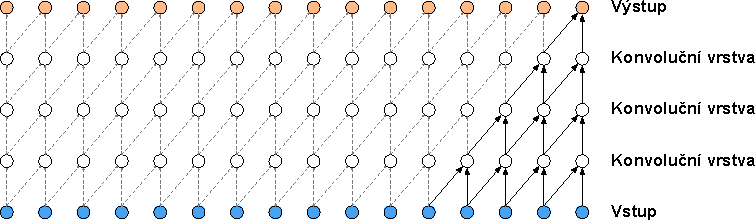
\includegraphics{../img/wavenet_konvoluce}
\caption{Vrstvení obyčejných konvolucí s lineárně rozšiřovaným dosahem, obrázek převzat z \cite{Oord2016}.}
\label{obr:wavenet_conv}
\end{figure}

\begin{figure}[h]\centering
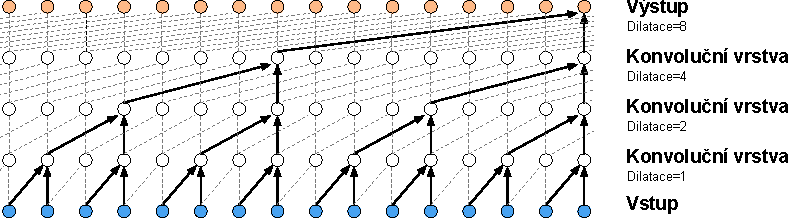
\includegraphics{../img/wavenet_dilatace_konvoluce}
\caption{Vrstvení dilatovaných konvolucí s exponenciálně rozšiřovaným dosahem, obrázek převzat z \cite{Oord2016}.}
\label{obr:wavenet_dilated}
\end{figure}

Síť se pro \emph{Music Information Retrieval} úlohy od svého zveřejnění příliš neuchytila. Její použití se v oblasti hudby se omezuje na generativní úlohy (\cite{Hawthorne2018a}, \cite{Yang2017}, \cite{Engel2017} a další), případně pro \uloha{source-separation} \citep{Stoller2018}. Jediný publikovaný pokus s použitím architektury WaveNet pro příbuznou úlohu kompletního automatického přepisu podnikli \cite{Martak2018} s použitím datasetu \dataset{MusicNet}. Jejich model však netestovali na standardních evaluačních datasetech ze soutěže MIREX, tudíž není zřejmé, jakých výsledků v porovnání s existujícími metodami autoři dosáhli.



% TODO: přidat schéma sítě z Martak2018

\subsection{Baseline na základě \cite{Martak2018}}

Pro srovnání spustíme architekturu popsanou ve zmíněném článku pro úlohu extrakce melodie. Jelikož byla architektura zamýšlena pro dataset MusicNet, který obsahuje celý přepis skladeb do MIDI not, výstupem jsou diskrétní noty. Jak jsme zjistili v předchozím experimentu na architektuře CREPE, hrubá diskretizace výrazně zhoršuje přesnost výsledků, upravíme proto architekturu tak, aby měla výstupní distribuce jemnější rozlišení.

% výsledek bude
% smooth labels, smoothing 0.18
% omezený rozsah
% batchsize 8
% adam opt --iterations 100000 --learning_rate_decay_steps 10000 --learning_rate_decay 0.8 
% last layer:
% avgpool_p5_s5_Psame--conv_f180_k16_s4_Psame_arelu--conv_f360_k64_s8_Psame
\subsection{Vliv počtu filtrů dilatačních vrstev}

Jedním ze zásadních faktorů ovlivňujících kapacitu sítě, je počet filtrů dilatačních vrstev a skip propojení. Podobně jako v případě architektury CREPE nalezneme vhodnou kapacitu sítě tak, aby nedocházelo k přeučení (overfitting) ani k nedoučení (underfitting) na trénovací množině.
Experimenty byly spuštěny na síti s dilatacemi $(1,2,4,8,16,\dots,512)$, s kernelem dilatovaných konvolucí šíčky 3, bez konvoluce pro předzpracování signálu



\subsection{Systematické prohledávání počtu dilatačních vrstev}

Způsob propojení dilatačních vrstev a jejich počet ovlivňuje 

\subsection{Vliv velikosti šířky kernelu dilatací}

\subsection{Vliv redukce skip propojení}

\subsection{Vliv návrhu posledních vrstev}

\subsection{Vliv velikosti první konvoluce}
